\input{../../templates/latex-template/main.tex}
\usepackage{pdflscape}

% overwrite for each document:
\def\sepmdocumentname{Projektendbericht}
\def\sepmauthors{Johannes Buchner, Simon Wallner}
\def\sepmreview{}
\def\sepmexecutivesummary{Abgabebericht zum Projektende von Jake}
% these are lines that are injected into the changelog table
\def\sepmchangeloglines{
1 & 21.3.2009 & Johannes Buchner & Dokument erstellt \\
2 & 22.3.2009 & Simon Wallner & Review \\
\hline
% repeat
}
\def\subfileinclude{
% your subsites
\input{intro.tex}
%\input{gantt.tex}
% and more
}

\sepmstart


\usepackage{pdflscape}

% overwrite for each document:
\def\sepmdocumentname{Projektendbericht}
\def\sepmauthors{Johannes Buchner, Simon Wallner}
\def\sepmreview{}
\def\sepmexecutivesummary{Abgabebericht zum Projektende von Jake}
% these are lines that are injected into the changelog table
\def\sepmchangeloglines{
1 & 21.3.2009 & Johannes Buchner & Dokument erstellt \\
2 & 22.3.2009 & Simon Wallner & Review \\
\hline
% repeat
}
\def\subfileinclude{
% your subsites
\setcounter{chapter}{1}
\section{Status}
Das Projekt Jake konnte nach verlängerter Entwicklungszeit fertiggestellt werden.

\section{Komponenten}
An den Komponenten \emph{FSS, ICS, ICS-XMPP} mussten lediglich kleine Änderungen und Bugfixes vorgenommen werden. 
Die großen Arbeitspakete seit dem letzten Bericht betrafen \emph{Core} und \emph{GUI}.

\subsection{Domainobjects, Datenbank}
Sämtliche Domainobjekte wurden von Johannes im Februar reviewed und überarbeitet um eine darauf aufbauende Weiterentwicklung zu ermöglichen. Ebenso wurden die DAOs getestet und fertigimplementiert. 

\subsection{JakeCommander}
Zum Testen und für einen Servermodus wurde eine durch Kommandozeile ansprechbare Implementierung geschrieben, die die meisten Use-Cases abdeckt.


\subsection{Core}
Die Use-Cases wurden fertigimplementiert, und die Übertragungs- und Synchronisationslogik konnte fertiggestellt werden.


\section{GUI}
Am GUI mussten keine Konzepte geändert werden, lediglich die Implementierung der Use-Cases wurde vervollständigt und poliert.


\section{Neuerungen}
Noch zu notieren wäre, ein interessantes Hibernate-Problem, dass lediglich eine Hibernate-Datenbankverbindung an einen Thread gebunden werden kann. Daher wurden alle Datenbankaufrufe in einen Dispatcherthread ausgelagert, der alle Datenbankanfragen pro Datenbank ausführt.

Zur Verbesserung der Performance wurde ein Cachingsystem entworfen, dass in verschiedenen Granularitäten Daten gecacht und aktualisiert werden können.


\section{Abschließende Bemerkungen}
Das Projekt Jake erreichte mit etwa 60.000 Codezeilen nach 2000 Arbeitsstunden mit den ausgereiften Projekten Checkstyle, Cobertura oder Log4J vergleichbare Größe.

Obwohl uns das Projekt Strapazen abverlangte, sind wir doch mit dem produzierten Ergebnis zufrieden.

\section{Anhänge}
\begin{itemize}
\item Gantt-Diagramm
\end{itemize}



%%\section{Inhalt}
%Noch mehr Inhalt ...


\begin{landscape}
\thispagestyle{empty}
\marginparsep = 1cm
%	\marginparwidth = 2cm
%\setlength{\leftmargin}{0.3cm}
%\setlength{\topmargin}{0.3cm}
%\setlength{\hoffset}{0.3cm}
%\setlength{\voffset}{0.3cm}
\oddsidemargin=1cm
\voffset=2.5cm
%\topmargin = 0.4cm
%\hoffset = 0cm
%\voffset = 0cm
\section{aktualisiertes Gantt-Diagramm}
\includegraphics[width=1.15\textwidth]{ase-gantt.png}
\end{landscape}

% and more
}

\sepmstart


\usepackage{pdflscape}

% overwrite for each document:
\def\sepmdocumentname{Projektendbericht}
\def\sepmauthors{Johannes Buchner, Simon Wallner}
\def\sepmreview{}
\def\sepmexecutivesummary{Abgabebericht zum Projektende von Jake}
% these are lines that are injected into the changelog table
\def\sepmchangeloglines{
1 & 21.3.2009 & Johannes Buchner & Dokument erstellt \\
2 & 22.3.2009 & Simon Wallner & Review \\
\hline
% repeat
}
\def\subfileinclude{
% your subsites
\setcounter{chapter}{1}
\section{Status}
Das Projekt Jake konnte nach verlängerter Entwicklungszeit fertiggestellt werden.

\section{Komponenten}
An den Komponenten \emph{FSS, ICS, ICS-XMPP} mussten lediglich kleine Änderungen und Bugfixes vorgenommen werden. 
Die großen Arbeitspakete seit dem letzten Bericht betrafen \emph{Core} und \emph{GUI}.

\subsection{Domainobjects, Datenbank}
Sämtliche Domainobjekte wurden von Johannes im Februar reviewed und überarbeitet um eine darauf aufbauende Weiterentwicklung zu ermöglichen. Ebenso wurden die DAOs getestet und fertigimplementiert. 

\subsection{JakeCommander}
Zum Testen und für einen Servermodus wurde eine durch Kommandozeile ansprechbare Implementierung geschrieben, die die meisten Use-Cases abdeckt.


\subsection{Core}
Die Use-Cases wurden fertigimplementiert, und die Übertragungs- und Synchronisationslogik konnte fertiggestellt werden.


\section{GUI}
Am GUI mussten keine Konzepte geändert werden, lediglich die Implementierung der Use-Cases wurde vervollständigt und poliert.


\section{Neuerungen}
Noch zu notieren wäre, ein interessantes Hibernate-Problem, dass lediglich eine Hibernate-Datenbankverbindung an einen Thread gebunden werden kann. Daher wurden alle Datenbankaufrufe in einen Dispatcherthread ausgelagert, der alle Datenbankanfragen pro Datenbank ausführt.

Zur Verbesserung der Performance wurde ein Cachingsystem entworfen, dass in verschiedenen Granularitäten Daten gecacht und aktualisiert werden können.


\section{Abschließende Bemerkungen}
Das Projekt Jake erreichte mit etwa 60.000 Codezeilen nach 2000 Arbeitsstunden mit den ausgereiften Projekten Checkstyle, Cobertura oder Log4J vergleichbare Größe.

Obwohl uns das Projekt Strapazen abverlangte, sind wir doch mit dem produzierten Ergebnis zufrieden.

\section{Anhänge}
\begin{itemize}
\item Gantt-Diagramm
\end{itemize}



%%\section{Inhalt}
%Noch mehr Inhalt ...


\begin{landscape}
\thispagestyle{empty}
\marginparsep = 1cm
%	\marginparwidth = 2cm
%\setlength{\leftmargin}{0.3cm}
%\setlength{\topmargin}{0.3cm}
%\setlength{\hoffset}{0.3cm}
%\setlength{\voffset}{0.3cm}
\oddsidemargin=1cm
\voffset=2.5cm
%\topmargin = 0.4cm
%\hoffset = 0cm
%\voffset = 0cm
\section{aktualisiertes Gantt-Diagramm}
\includegraphics[width=1.15\textwidth]{ase-gantt.png}
\end{landscape}

% and more
}

\sepmstart



% overwrite for each document:
\def\sepmdocumentname{Projektvorschlag}
\def\sepmauthors{Johannes Buchner}
\def\sepmreview{}
\def\sepmexecutivesummary{Das Projekt soll Benutzern ermöglichen, gemeinsam an einem Dateienpool zu arbeiten und Notizen bzw. Ankündigungen zu organisieren. Der vorliegende Projektvorschlag führt in die technische Planung und Arbeitsplanung ein. }
% these are lines that are injected into the changelog table
\def\sepmchangeloglines{
1 & 11.04.2008 & Johannes Buchner & Dokument erstellt \\
\hline
%2 & 17.04.2008 & Peter Steinberger & Arbeitsziele und Projektplan eingefügt  \\
%\hline
%2 & 12.04.2008 & Johannes Buchner, Simon Wallner & Phasen einführen \\
%\hline
%3 & 12.04.2008 & Johannes Buchner & Deckblatt, Konfliktbewältigung, Domänenmodell \\
%\hline
%4 & 13.04.2008 & Dominik Dorn & Überarbeitung Programmdefinition \\
%\hline
%5 & 17.4.2008 & Simon Wallner & Abschnitt Informationswesen eingefügt\\
%\hline
% repeat
}

\def\subfileinclude{
% your subsites
\setcounter{chapter}{1}
\chapter{Projektauftrag}
\thispagestyle{fancy}

% Projektname, Arbeitstitel
% Beschreibung der Projektidee wie im Projektvorschlag nur noch etwas ausführlicher, gestützt auf unsere Features/Use Cases/Assumptions

\section{Projektbeschreibung}
Die Weiterentwicklung von \sepmprojectname wird es Projektgruppen erlauben, über das Internet an Projektordnern zu arbeiten.

\sepmprojectname soll den Grundstein für eine Plattform legen, die es erlaubt, über ein Netzwerk (z.B. das Internet) gemeinsam an Dateien beliebigen Formats zu arbeiten. Es soll ein Fat Client entwickelt werden, der alle Funktionen der im Projekt definierten Synchronisationsschnittstelle benutzt, die Implementierung der Netzwerk- und Synchronisationsservices ist aber erst in darauf folgenden Ausbauphasen in Form eigenständiger Projekte geplant. Änderungen an Dateien sollen vom Programm erkannt werden und mit Hilfe der Synchronisations- und Netzwerkservices an andere User propagiert werden. In diesem Projekt soll nur die Phase 1 der folgenden Phaseneinteilung realisiert werden.

\subsection{Phase 1, Fat Client}
In dieser Phase wird das Programm als Fat Client erstellt, dessen grafischen Oberfläche die vollständige Nutzbarkeit der unten aufgeführten Features benutzbar macht. 
Die Netzwerkkommunikation zwischen verschiedenen Clients soll mithilfe eines Mock-Service simuliert werden. Dieser Service wird in dieser Phase die Zusammenarbeit mit anderen Clients simulieren, wodurch die Funktionalität des Programmes getestet werden kann. Neben diesem Mock-Service, welches die Netzwerkservices der Anwendung kapselt, wird zusätzlich noch ein Synchronisationsinterface erstellt, welches es erlaubt, den Vorgang der Synchronisation zwischen den Clients, auf verschiedene Weisen zu implementieren.
Die Synchronisation soll in dieser Phase ebenfalls mithilfe eines Mock-Services realisiert werden. Die Netzwerk- und Synchronisations-Mock-Services können dann in möglichen späteren Projektphasen durch entsprechende Implementierungen (z.B. XMPP für das Netzwerkservice) ersetzt werden. Die für die Synchronisation notwendigen Elemente der Benutzeroberfläche sollen aber bereits in dieser Phase erstellt und an die entsprechenden Schnittstellen gebunden werden. 

\subsubsection{Aufgaben des Networkservice}
Authentifizierung der Benutzer
Netzwerkverbindung zwischen den Clients
Austausch von Nachrichtenpaketen zwischen den Clients
Datenaustausch zwischen den Clients

\subsubsection{Aufgaben des Synchronisationsservice}
Abholen von Dateiversionen, die andere Projektmitglieder erstellt haben
Verbreiten eigener Änderungen
Abgleich von Dateiversionen zwischen Clients
Erkennen von Dateikonflikten
\subsection{Phase 2, Networking / Synchronisation}
Die Mock-Services werden durch konkrete Implementierungen des Networkservice und des Synchronisationsservice ersetzt. Für das Networkservice ist zur Zeit eine Lösung auf Basis des XMPP-Protokolles angedacht. Durch eine generischen Definition der Schnittstellen in Phase 1 kann dies aber auch mit beliebigen anderen Technologien erfolgen.
\subsection{Phase 3, Service Sharing}
In dieser Phase ist das zur Verfügung stellen lokaler Services (z.B. Printer Server) zwischen den Projektmitgliedern geplant.

\subsection{Projektabgrenzung}
% Dinge, die man falscherweise vom Projekt erwarten könnte
% Damit man sich nicht am Ende wundert.
Es wird nur die erste Phase implementiert, was das Programm nur lokal benutzbar macht, und andere Systeme durch Mock-Services simuliert. 
Es ist nicht möglich, "live" gleichzeitig an einem Dokument zu arbeiten (wie etwa Gobby oder Google Apps).
Es werden keine alten Versionen/Revisionen behalten, die wiederhergestellt werden könnten.
Es wird kein automatisches Mergen (etwa von Textdateien) implementiert, da auf Benutzungsumgebungen fokussiert wird, die binäre bzw. proprietäre Formate verwenden.







%      Am Projekt beteiligte Personen und ihre Verantwortlichkeiten. Dies beinhaltet auch unsere Auftraggeber (Tutor, Assistent) und unsere Stakeholder (User)
%      Auflistung der Teammitglieder mit Rolle und Kontaktdaten

\section{Arbeitsstruktur}
\subsection{Auftraggeber}
\begin{tabular}{ | l | l | p{3.5cm} | p{4cm} |}
\hline
\textbf{Rolle} & \textbf{Name} & \textbf{Mail} & \textbf{Telefon} \\
\hline
betreuender Assistent & Marco Zapletal & marco@ ec.tuwien.ac.at & 01 588 01 - 18822 \\
\hline
betreuender Tutor & Anton Matzneller & anton.matzneller@ googlemail.com &  \\
\hline
\end{tabular}

\subsection{Auftragnehmer}
\begin{tabular}{ | l | l | p{5.5cm} | p{1.7cm} | l | l |}
\hline
\textbf{Rolle} & \textbf{Name} & \textbf{Mail} & \textbf{Telefon} & \textbf{Matr.} & \textbf{KZ} \\
\hline
TK & Simon Wallner & me@simonwallner.at & 0699 11 55 24 51 & 0625104 & 532 \\
\hline
TKS & Peter Steinberger & peter.steinberger@ student.tuwien.ac.at & 0664 918 37 24 & 0626583 & 534 \\
\hline
TA & Chris Sutter & chris@doublesignal.com & 0660 61 61 808 & 0505267 & 534 \\
\hline
TAS & Philipp Knobelspies & e0547943@student.tuwien.ac.at & 0699 81 39 93 84 & 0547943 & 534 \\
\hline
Test & Dominik Dorn & dominik.dorn@gmail.com & 0669 12 64 79 73 & 0626165 & 534 \\
\hline
Doku & Johannes Buchner & e0625457@student.tuwien.ac.at & 0699 10 04 33 47 & 0625457 & 534 \\
\hline
\end{tabular}

\subsection{Main Stakeholder}
Personen, die geringe bis mittlere Computererfahrung haben und in Projekten Dateien verschiedener Formate bis zu einer Größe von ca 5 MB austauschen und zusammen bearbeiten möchten. Die Projektmitglieder sind während der Arbeit an dem Projekt die meiste Zeit online.
\subsection{Modellszenario}

Eine Projektgruppe, deren 3-12 Mitglieder auf verschiedenen Rechnern arbeiten, die vorwiegend online sind und gemeinsam 5-100 Dateien benutzen. Eine einzelne Datei wird dabei meist nur von einem Benutzer gleichzeitig bearbeitet.

%    Beschreibung der Ziele die unser Projekt verfolgt. Dabei werden die einzelnen Ziele in Kategorien zusammengefasst, wie z.B. betriebswirtschaftliche Ziele, funktionale Ziele, Marketing-Ziele, soziale Ziele, Umfeldziele
%    Angabe der Lieferkomponenten, die komponenten die an den Kunden ausgeliefert werden
%    Angabe weiterer Komponenten die nicht an den Kunden ausgeliefert werden. technische Doku, interne Doku, …

\section{Arbeitsziele}

\subsection{Betriebswirtschaftliche Ziele}
\begin{itemize}
\item Die Zeit die für das Verteilen, Speichern und Zusammenführen von verschiedenen Versionen eines Dokuments aufgewendet wurde kann nun für andere Tätigkeiten verwendet werden.
\item Durch Meta-Tags der Datenobjekte wird die Übersichtlichkeit verbessert, was die Effizienz der Mitarbeiter eines Projektes erhöht.
\end{itemize}

\subsection{Funktionale Ziele}
\begin{itemize}
\item Durch den Einsatz der Applikation wird es einfacher ad-hoc neue Dokumente der Projektgruppe zur Verfügung zu stellen oder Aktualisierungen an bestehenden zu Propagieren. Da dieser Austausch nicht mehr per Mail geschieht wird die Übersicht über die Daten erhöht, und Versionskonflikte mit alten lokalen Versionen stark verringert.

\item Durch den Einsatz der Applikation können Aktualisierungen an Dateien anderen Projektmitgliedern schneller zugänglich gemacht werden. Da die Projektmitglieder, sofern möglich, immer die aktuellsten Versionen zur Verfügung haben, ist eine dynamischere Arbeitsweise möglich, die stärker auf Zusammenarbeit setzt.

\item Da der Dateiaustausch nicht mehr händisch per Mail geschieht müssen alte Versionen nicht mehr manuel organisiert werden, wodurch ein Versionschaos leichter vermieden werden kann.

\item Treten dennoch Datei-Versionskonflikte auf, wird der Benutzer von der Applikation bei deren Lösung unterstützt, wodurch diese einfacher zu handhaben sind und weniger Zeit in Anspruch nehmen.

\end{itemize}

\subsection{Soziale Ziele}
\begin{itemize}
\item Durch den einfacheren Datenaustausch wird die engere Zusammenarbeit der Projektmitglieder unterstützt.
\end{itemize}

\subsection{Lieferkomponenten}
Bei Projektabschluss werden folgende Komponenten übermittelt:
\begin{itemize}
\item die voll funktionale Applikation laut Anforderungsspezifikation als lauffähiges .jar Paket (benötigt JRE 1.6).
\item Benutzerhandbuch
\item Anforderungsspezifikation
\item Source Code
\item technische Dokumentation
\end{itemize}

Die gesamte Dokumentation wird in einer Website zur Verfügung gestellt. Das Programm sowie die Dokumentation werden in englischer Sprache verfasst.

\subsection{Weitere Komponenten}
\begin{itemize}
\item Projektvorschlag
\item Projektauftrag
\item Projekt-Wiki
\item Dokumente der internen Projektorganisation
\item Artefakte des laufenden Projektmanagement
\item Stundenlisten
\item Projekttagebuch
\item Protokolle
\end{itemize}

% funktionale Anforderungen, Anwendungsfälle
%    Eine Liste von funktionalen Anforderungen oder eine Liste von User-Level Use Cases. Dabei sind nicht die ausführlichen Use Cases selbst gemeint (die kommen erst später) sondern lediglich gut beschreibende one-liner, eine Weiterführung der Featureliste. z.B. Datei zum Projektpool hinzufügen, neues Projekt erstellen, neues Projektmitglied hinzufügen

\section{Use Cases}
% Es soll entweder eine Liste von Anforderungen oder eine Liste von (User-Level)
% Anwendungsfällen erstellt werden. Dabei soll die Featureliste aus dem
% Projektvorschlag hilfreich sein. Egal ob Anwendungsfälle oder Anforderungen, beide
% können Gewichtet und aufgeteilt werden um eine Entscheidungsgrundlage für das
% Arbeitsprogramm und die WBS zu erstellen. (z.B. Need-to-Have, Nice-to-Have)
% BEISPIEL
% Anforderungen: User Interface soll Eingabemasken zur Verwaltung von Studenten
% und Prüfungen implementieren. Studentenlisten sollen über einen grafischen
% Dateiauswahl- bzw. Dateispeicherdialog als XML geöffnet und gespeichert werden
% können.
% Anwendungsfälle: Studenten verwalten/exportieren, Prüfung anmelden/absolvieren

% Hier bitte ENTWEDER alles Anwendungsfälle ODER alles Features schreiben
% nicht mischen!

% Dies sind Anwendungsfälle:
\begin{itemize}
\item Projekte verwalten
\item Projektmitglieder verwalten/einladen
\item Dateien/Ordner zum Projektdatenpool hinzufügen
\item Dateien/Ordner aus dem Projektdatenpool entfernen
\item Datei aus dem Projektdatenpool zur Bearbeitung mit einer externen Applikation öffnen
\item Notizen organisieren
% Was hat das Projekt für Metadaten ??? Eher weglassen
\item Metadaten des Projekts verwalten % <--
% 
\item Metainformationen der Dateien und Notizen verwalten
\item Metadaten der Projektmitglieder verwalten
\item Lokale Änderungen an Projektmitglieder propagieren
\item Aktualisierte Versionen von Projektmitgliedern holen
\item Versionskonflikt lösen
\item Nachrichten an Projektmitglieder schicken
\item Nachrichten empfangen
\end{itemize}
% Komponentendiagramm des Projektes
\section{Komponentendiagramm}

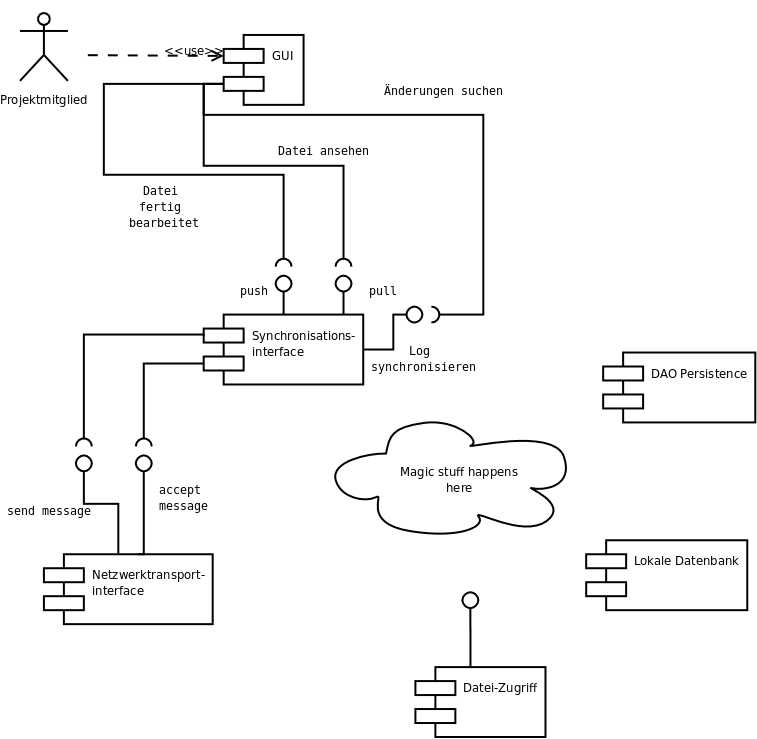
\includegraphics[width=0.98\textwidth]{../uml/component_diagram.png}

Das Projekt ist in folgende 6 Komponenten aufgeteilt:

% Wie man sieht habe ich sehr viel dazugeschrieben. Allgemein ist mein Verständnis von einer Komponente das, dass ich von ihr wissen will, wofür ich sie nutzen kann und was sie mir für Services anbietet. ~simon

% Es sollen zuerst die Aufgaben jeder Komponente beschrieben.
% Danach kann auf Verbindung zu anderen Komponenten eingegangen werden: Nicht durch Abläufe, es sollen die Beziehungen beschrieben werden
% Die Beziehung ist, dass der Core immer die Kontrolle hat, aber dass er eben auch auf Callbacks/Events von den anderen Komponente wartet
% Nicht die internen Abläufe beschreiben, und bei allen Komponenten auf gleichem Detailniveau bleiben. 
% ~johannes


\subsection{Core}
In der Core-Komponente befindet sich die Business Logic der Applikation. Der Core steuert die Funktionalität und die anderen Komponenten, wartet aber auch auf Events/Callbacks von den anderen Komponenten. 
Dies kann etwa das Drücken eines Buttons sein, die Änderung einer Datei im Dateisystem oder eine Nachricht von einem anderen Client. Die jeweilige Komponente wirft einen Event/Callback, den der Core empfängt.

\subsection{Graphical User Interface}
Die grafische Benutzeroberfläche, mit der der Endanwender arbeitet, ermöglicht Zugriff auf alle von der ``Core''-Komponente für Endbenutzer zur Verfügung gestellten
Funktionalitäten.

% Persistence NICHT Database Persistence, es ist nicht festgelegt dass wir eine Datenbank verwenden ~simon
\subsection{Persistence} 
Die Persistence Komponente abstrahiert den Zugriff auf die Daten, die für den Betrieb gespeichert werden müssen. Diese umschließen nicht die Dateien. Es wird das Konzept des Data Hiding umgesetzt, wodurch erreicht werden kann, dass die anderen Komponenten nur auf definierte Weise die Daten verwenden. Für die Speicherung der Daten kann eine relationale Datenbank verwendet werden.

\subsection{Synchronisation Services}
Die Synchronisationskomponente ist für die Verteilung von Änderungsinformationen und Dateninhalten an andere Projektmitglieder/Clients zuständig. 

\subsection{File System Services}
Die File System Services kapselt den Zugriff auf Dateien im Dateisystem. Außerdem kann diese Komponente durch entsprechende Strategien feststellen, ob Dateien geändert wurden oder in die Projektordnerstruktur kopiert wurden und dies dem Core mitteilen, welcher wiederum entsprechende Aktionen veranlasst.

\subsection{Interclient Communication} 
Der Interclient Communication Service kapselt die vollständige Kommunikation zwischen den Clients (über das Netzwerk) und gibt die entsprechenden Nachrichten an den Core weiter. So ist es leicht möglich, verschiedene Netzwerk-backends (z.B. XMPP oder RMI) zu unterstützen, welche für den Core und somit für den Benutzer transparent sind. Außerdem wird die Authentifizierung der Nutzer in dieser Komponente durchgeführt. 
% Ich habe bei Client Authentifizierung ein schlechtes Gefühl. Wenn wir nicht mit XMPP arbeiten, wie werden die Clients dann Authentifiziert? ~simon
% ja. ~johannes
% grob
%    Festlegung der Meilensteine
%    Erstellung eines ersten groben Projektplans der alle Meilensteine mit dem zu erwartenden Fertigstellungszeitpunkt beinhaltet.


\section{Projektplan}
%% TODO: Die Daten mit WBS abgleichen, ich hab jetzt nur Daten gestreut
%% TODO: Stunden eintragen
\begin{tabular}{ | p{6cm} | p{4cm} | l | }
\hline
\textbf{Meilenstein / Tätigkeit} & \textbf{Termin} & \textbf{Personalaufwand} \\
\hline
Projektstart & 12.04.2008 & \\
\hline
Anforderungsanalyse abgeschlossen & 18.04.2008 & \\
\hline
Schnittstellendefinition abgeschlossen  & 30.04.2008 & \\
\hline
Technische Entwurfsphase abgeschlossen & 30.04.2008 & \\
\hline
Beginn Implementierung & 01.05.2008 & \\
\hline
Abschluss der Schnittstellenimplementierung & 13.05.2008 & \\
\hline
50\% der Implementierung abgeschlossen & & \\
\hline 
Abschluss der UI-Implementierung & & \\
\hline
Feature Complete & & \\
\hline
Fertigstellung und Release & 17.6.2008 & \\
\hline
Projektabschluss: Abgabe aller Artefakte, Applikation, Doku; Ende der Übung& 20.6.2008 & \\
\hline
\end{tabular}


% Aufteilung unseres Projekts in bit-sized-chunks. Für diese Teilaufgaben wird dann der Aufwand geschätzt

\section{Arbeitsprogramm, Work Breakdown Structure}

\begin{tabular}{ | l | p{8cm} | p{2cm}|p{2cm}|p{2cm}|}
\hline
\textbf{Nr.} & \textbf{Phase / Outcome} & \textbf{Beginn / Woche}& \textbf{Ende / Woche}& \textbf{Aufwand / Std.} \\
\hline
1 & \textbf{Projektstart}                      & \textbf{1} & \textbf{2} & \textbf{68} \\
\hline
1.1& Rollenverteilung                  &1 &2 &2 \\
\hline
1.2 &Dokumentationsrichtlinien         &1 &2 &4 \\
\hline
1.3 &Termine für laufende Meetings     &2 &2 &4 \\
\hline
1.4 &Meilensteine                      &2 &2 &3 \\
\hline
1.5 &Projektauftrag                    &2 &2 &55 \\
\hline
2&\textbf{Anforderungsanalyse}               &\textbf{2} &\textbf{4}&\textbf{38}  \\
\hline
2.1 &Features/funktionale Anforderungen&2 &2 &10 \\
\hline
2.2 &Use Cases                         &2 &3 &7  \\
\hline
2.3 &Use Case Diagramm                 &3 &3 & 3 \\
\hline
2.4 &Assumptions                       &2 &4 & 12 \\
\hline
2.5 &nichtfunktionale Anforderungen    &2 &2 & 3 \\
\hline
2.6 &Domain Model                      &1 &2 & 3 \\
\hline
3&\textbf{technischer Entwurf}              &\textbf{2} &\textbf{4} & \textbf{50}  \\
\hline
3.1 &Komponenten                       &2 &4 & 10 \\
\hline
3.2 &Komponentendiagramm               &2 &4 & 4 \\
\hline
3.3 &Interfaces                        &3 &4 & 10 \\
\hline
3.5 &Klassendiagramm                   &3 &4 & 8 \\
\hline
3.6 &Coding Guidelines                 &3 &4 & 2 \\
\hline
3.7 &ER/EER                            &2 &4 & 4 \\
\hline
3.8 &Systemarchitektur                 &2 &4 & 12 \\
\hline
4 &\textbf{User Interface}                   &\textbf{4} &\textbf{5} & \textbf{30} \\
\hline
4.1 &Grobentwurf                       &4 &5 & 10 \\
\hline
4.2 &Prototyp                          &4 &5 & 20 \\
\hline
5 &\textbf{Implementierung}                 & & & \textbf{400} \\
\hline
5.1 &Implementierung Interfaces        &4 &6 & 20 \\
\hline
5.2 &Implementierung Komponenten       &5 &9 & 110 \\
\hline
5.3 &Implementierung UI                &5 &9 & 40 \\
\hline
5.6 &Implementierung Programmlogik     &5 &9 & 230 \\
\hline
6 &\textbf{Testen}                           &\textbf{4} &\textbf{9} & \textbf{68} \\
\hline
6.1 &Test Guidelines                   &4 &5 & 8 \\
\hline
6.2 &Testplan                          &5 &7 & 5 \\
\hline
6.2 &Testen                            &5 &9 & 50 \\
\hline
6.3 &Testreport                        &9 &9 & 5 \\
\hline
\end{tabular}

\begin{tabular}{ | l | p{8cm} | p{2cm}|p{2cm}|p{2cm}|}
\hline
\textbf{Nr.} & \textbf{Phase / Outcome} & \textbf{Beginn}& \textbf{Ende}& \textbf{Aufwand / Std.} \\
\hline
7 &\textbf{Dokumentation}                   &\textbf{1} &\textbf{10} &\textbf{147}  \\
\hline
7.1 &Dokumentations-Guidelines         &1 &3 & 5 \\
\hline
7.2 &Review-Prozess Definition         &1 &3 & 4 \\
\hline
7.3 &technische Dokumentation          &3 &9 & 70 \\
\hline
7.4 &Projektmappe gedruckt + CD        &10 &10 & 8 \\
\hline
7.5 &User Manual                       &8 &9 & 20 \\
\hline
7.6 &Artefakte                         &1 &10 & 40 \\
8 &\textbf{Dokumente der Projektplanung}     &\textbf{1} &\textbf{11} &\textbf{105}  \\
\hline
8.1 & Statusberichte                &3 &11 & 20 \\
\hline
8.2 &Stundenliste                      &1 &11 & 8 \\
\hline
8.3 &Projekttagebuch                   &2 &11 & 10 \\
\hline
8.4 &Protokolle                        &2 &11 & 20 \\
\hline
8.5 &Meilenstein Trendanalyse          &3 &11 & 8 \\
\hline
8.6 &Projektplan fein/Gantt            &3 &11 & 10 \\
\hline
8.7 &Risikoanalyse                     &3 &4 & 6 \\
\hline
8.9 &WBS                               &2 &2 & 8 \\
\hline
8.10 &Projektplan grob                 &2 &2 & 5 \\
\hline
8.11 &Workload Erhebung                &2 &11 & 10 \\
\hline
\hline
& \textbf{Gesamt} & & & \textbf{900} \\
\hline
\hline
\end{tabular}

% Dieser Teil korrespondiert mit der Projektbeschreibung. 
% Er legt fest was unser Projekt nicht ist, und was daher auch nicht implementiert wird.

\section{Projektabgrenzung}
\begin{itemize}
  \item Im Rahmen der Laborüubung SEPM wird nur die erste Phase laut Projektbeschreibung implementiert. Die konkrete Implementierung der Netzwerk- und Synchronisationsfunktionalität erfolgt erst in einer späteren Projektphase und wird in der ersten Phase durch Mock-Objekte simuliert.
  \item Es ist nicht möglich, in Echtzeit gleichzeitig an einem Dokument zu arbeiten (wie etwa in Gobby oder Google Apps).
  \item Es soll kein SCM oder Versionsmanagement implementiert werden. Alte Versionen von Dateien werden nicht behalten und sind daher auch nicht wiederherstellbar.
  \item Da der Fokus auf Nutzungsumgebungen liegt, die primär binäre beziehungweise proprietäre Formate verwenden, soll kein automatisches Mergen (etwa von Textdateien) implementiert werden.
  \item
\end{itemize}
% Proforma Schätzung des Personalaufwandes

\section{Kostenabschätzung}

Da die benötigte Hardware schon vorhanden ist und keine Software zugekauft werden muss, fällt bei der Entwicklung lediglich Personalaufwand als Kosten an. Dieser wird mit etwa 900 Personenstunden veranschlagt.



%Informationswesen/Dokumentation
%   Interne Kommunikation, Dokumentation, Dokumentationsrichtlinien, Reviewprozess


\section{Informationswesen/Dokumentation}
\subsection{Interne Kommunikation}
Zur internen Kommunikation wird ein eigens eingerichtetes Wikisystem verwendet.
Ankündigungen und wichtige Mitteilungen werden über eine Mailingliste verteilt. 
Die gesamte Projektgruppe trifft sich mindestens einmal pro Woche zu einem ein- bis eineinhalbstündigen Meeting. 
Die Agenda für die Meetings wird zuvor im Wiki bekanntgegeben und kann dort diskutiert werden. 

\subsection{Externe Kommunikation}
Die externe Kommunikation wird während der Übung über regelmäßig stattfindende Review-Meetings sowie über Email-Kommunikation mit unserem Tutor und Assistenten geführt.

\subsection{Organisatorische Dokumentation}
Die organisatorische Dokumentation des Projekts wird über das Wiki abgewickelt. 
Protokolle, Stundenlisten, Projekttagebuch, etc. werden während der Dauer der Übung laufend aktualisiert.

\subsection{Technische Dokumentation}
Die gesamte technische Dokumentation und Spezifikation wird über Maven abgewickelt. 
Dies umfasst Dokumente der technischen Planung, Dokumente der Anforderungsspezifikation, 
Dokumente der Qualitätssicherung, Dokumentation auf Codeebene, Endbenutzer-Dokumente, etc.

Sämtliche technischen Spezifikationen werden in Englisch verfasst.

% and more
}
\sepmstart

